\chapter{Extremal Combinatorics}

\lecture{1}{15 Sep.}{}

\begin{question}
    How large can a structure be if it satisfies certain properties?
\end{question}

\begin{eg}[Mantel, 1907]
    How many edges can a graph in \(n\) vertices have if it doesn't contain a triangle?
\end{eg}

To show the answer is \(f(n)\), we need to do two things. 
\begin{enumerate}[(1)]
    \item Show there is a triangle-free graph on \(n\) vertices with \(f(n)\) edges. 
    \item Prove that any \(n\)-vertex graph with \(> f(n)\) edges must have a triangle.    
\end{enumerate} 

\begin{theorem}[Mantel, 1907]
    The largest \(n\)-vertex triangle-free graph has \(\left\lfloor \frac{n^2}{4} \right\rfloor\) edges.  
\end{theorem}

\begin{remark}
    The complete graph \(K_n\) on \(n\) vertices has \(\binom{n}{2} \thickapprox \frac{1}{2} n^2\) edges.   
\end{remark}

\begin{proof}[proof of Mantel's theorem]
    \hfill
    \begin{enumerate}[(1)]
        \item Bipartite graphs are triangle-free. Thus, we can split the vertices into two parts, take all edges between the parts. Suppose first part is of \(a\) vertices and the other one is of \(n - a\) vertices.
        \begin{center}
            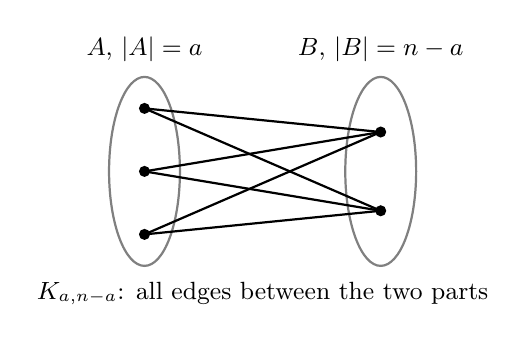
\begin{tikzpicture}[thick, every node/.style={font=\small}]
                \draw[gray] (0,0) ellipse (0.45 and 1.2);
                \draw[gray] (3,0) ellipse (0.45 and 1.2);
                \foreach \height [count=\index] in {0.8,0,-0.8}
                    \coordinate (left-\index) at (0,\height);
                \foreach \height [count=\index] in {0.5,-0.5}
                    \coordinate (right-\index) at (3,\height);
                \foreach \leftindex in {1,2,3}
                    \foreach \rightindex in {1,2}
                        \draw (left-\leftindex) -- (right-\rightindex);
                \foreach \index in {1,2,3} \fill (left-\index) circle (2pt);
                \foreach \index in {1,2} \fill (right-\index) circle (2pt);
                \node at (0,1.55) {$A$, $|A|=a$};
                \node at (3,1.55) {$B$, $|B|=n-a$};
                \node at (1.5,-1.55) {$K_{a,n-a}$: all edges between the two parts};
            \end{tikzpicture}
        \end{center}
        Note that this construction is triangle-free becuase given any three vertices, two fall in same part, and thus there is no edge between them. 
        Note that the number of edges is \(a(n - a) \le \left\lfloor \frac{n^2}{4} \right\rfloor\), where the equality holds iff \(a = \left\lfloor \frac{n}{2} \right\rfloor\) or \(\left\lceil \frac{n}{2} \right\rceil \).

        \begin{minipage}{\linewidth}
        \begin{note}
            Every bipartite graph is triangle-free, but a triangle-free graph need not be bipartite. For example, \(C_5\) consists of the five edges of a pentagon, with no diagonals, so it contains no triangle.

            To see why \(C_5\) is not bipartite, suppose that its vertices could be partitioned into two sets \(A\) and \(B\), with every edge joining different sets. Put the top vertex in \(A\); we can always exchange the names of the two sets to do this. Moving clockwise around the pentagon, each vertex must belong to the opposite set from the previous vertex. Thus the five vertices are forced to belong to
            \[
                A,\quad B,\quad A,\quad B,\quad A.
            \]
            But the last vertex is adjacent to the first vertex, and both are in \(A\), a contradiction. Hence no bipartition exists.
            \begin{center}
                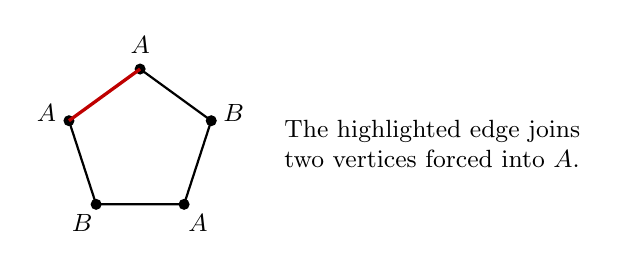
\begin{tikzpicture}[thick, every node/.style={font=\small}]
                    \foreach \index/\part in {1/A,2/B,3/A,4/B,5/A} {
                        \coordinate (cycle-\index) at ({90-72*(\index-1)}:0.95);
                        \fill (cycle-\index) circle (2pt);
                        \node at ({90-72*(\index-1)}:1.25) {$\part$};
                    }
                    \draw (cycle-1) -- (cycle-2) -- (cycle-3) -- (cycle-4) -- (cycle-5);
                    \draw[red!75!black, very thick] (cycle-5) -- (cycle-1);
                    \node[align=left, anchor=west] at (1.7,0)
                        {The highlighted edge joins\\two vertices forced into $A$.};
                \end{tikzpicture}
            \end{center}
            The labels \(A,B\) indicate the proposed parts, not vertex names. The red edge is an ordinary edge of \(C_5\), highlighted only to show the contradiction; this is not an edge-coloring problem.
        \end{note}
        \end{minipage}

        \item \hfill \begin{claim}
            If \(G\) is an \(n\)-vertex, triangle-free graph, then \(e(G) \le \left\lfloor \frac{n^2}{4} \right\rfloor\).   
        \end{claim}

        \begin{proof}[proof of claim]
            Let \(v \in V(G)\) be a vertex of maximum degree \(\Delta \). Since \(G\) is triangle-free, the neighborhood of \(v\) is independent (no edges).
            \begin{center}
                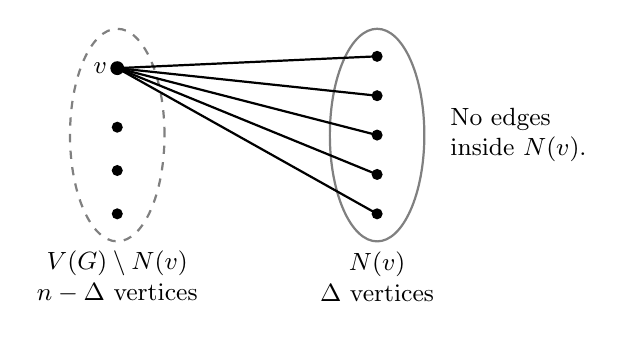
\begin{tikzpicture}[thick, every node/.style={font=\small}]
                    \draw[gray, dashed] (0,0) ellipse (0.6 and 1.35);
                    \draw[gray] (3.3,0) ellipse (0.6 and 1.35);
                    \coordinate (vertex) at (0,0.85);
                    \foreach \height in {1,0.5,0,-0.5,-1} {
                        \draw (vertex) -- (3.3,\height);
                        \fill (3.3,\height) circle (2pt);
                    }
                    \foreach \height in {0.1,-0.45,-1} \fill (0,\height) circle (2pt);
                    \fill (vertex) circle (2.5pt) node[left] {$v$};
                    \node[align=center] at (0,-1.8) {$V(G)\setminus N(v)$\\$n-\Delta$ vertices};
                    \node[align=center] at (3.3,-1.8) {$N(v)$\\$\Delta$ vertices};
                    \node[anchor=west, align=left] at (4.1,0) {No edges\\inside $N(v)$.};
                \end{tikzpicture}
            \end{center}
            Thus, every edge contains at least one vertex of \(V(G)\setminus N(v)\), where this set includes \(v\) itself. Thus,
            \begin{align*}
                e(G) \le \sum_{u: u \nsim v} \# \left\{ \text{edges containing } u  \right\} = \sum_{u: u \nsim  v} \deg (u) \le \sum_{u: u \nsim v} \Delta = \Delta (n - \Delta ) \le \left\lfloor \frac{n^2}{4} \right\rfloor.   
            \end{align*}      
        \end{proof}
    \end{enumerate}

    \begin{remark}
        Up to isomorphism, the unique \(n\)-vertex triangle-free graph with \(\lfloor n^2/4\rfloor\) edges is the balanced complete bipartite graph
        \[
            K_{\lfloor n/2\rfloor,\lceil n/2\rceil}.
        \]
        To prove uniqueness, suppose that \(G\) attains this bound. As in the proof above, choose a vertex \(v\) of maximum degree \(\Delta\), and write
        \[
            A=N(v),\qquad B=V(G)\setminus N(v).
        \]
        Then \(|A|=\Delta\), \(|B|=n-\Delta\), and \(A\) is independent because \(G\) is triangle-free. The inequalities in the proof become
        \[
            \left\lfloor\frac{n^2}{4}\right\rfloor
            =e(G)\le \sum_{u\in B}\deg(u)
            \le \Delta(n-\Delta)
            \le \left\lfloor\frac{n^2}{4}\right\rfloor.
        \]
        Since the first and last quantities agree, every inequality must be an equality. Each equality gives a structural restriction:
        \begin{enumerate}[(i)]
            \item \textbf{There are no edges inside \(B\).}
            Let \(e(B)\) denote the number of edges with both endpoints in \(B\). Since there are no edges inside \(A\), the degree sum over \(B\) counts every edge between \(A\) and \(B\) once and every edge inside \(B\) twice. Thus
            \[
                \sum_{u\in B}\deg(u)=e(G)+e(B).
            \]
            Equality \(e(G)=\sum_{u\in B}\deg(u)\) forces \(e(B)=0\). Both \(A\) and \(B\) are therefore independent, so \(G\) is bipartite with these parts.

            \item \textbf{Every possible edge between the parts is present.}
            Each \(u\in B\) has \(\deg(u)\le\Delta\). Equality
            \[
                \sum_{u\in B}\deg(u)=|B|\Delta
            \]
            forces \(\deg(u)=\Delta\) for every \(u\in B\); otherwise the sum would be strictly smaller. All neighbors of \(u\) lie in \(A\), which has exactly \(\Delta\) vertices. Hence every vertex of \(B\) is adjacent to every vertex of \(A\), giving \(G=K_{\Delta,n-\Delta}\).

            \item \textbf{The two parts are as equal in size as possible.}
            Finally, \(\Delta(n-\Delta)=\lfloor n^2/4\rfloor\). Using
            \[
                \Delta(n-\Delta)=\frac{n^2-(2\Delta-n)^2}{4},
            \]
            we obtain \(2\Delta-n=0\) when \(n\) is even, and \(2\Delta-n=\pm1\) when \(n\) is odd. Thus the part sizes are \(\lfloor n/2\rfloor\) and \(\lceil n/2\rceil\).
        \end{enumerate}
        Conversely, this balanced complete bipartite graph is triangle-free and has exactly \(\lfloor n^2/4\rfloor\) edges, as shown in the construction. This proves both extremality and uniqueness up to relabeling vertices.
    \end{remark}
\end{proof}

\begin{definition}
    The \vocab{Ramsey number \(R(k)\)} is the smallest \(n\) s.t. every red-/blue-coloring of the edges of \(K_n\) contains a monochromatic copy of \(K_k\).    
\end{definition}

\begin{theorem}[Ramsey, 1930]
    \(R(k)\) is finite. 
\end{theorem}

We can simply show \(R(1) = 1, R(2) = 2\), and for \(R(3)\), it is a little harder to show \(R(3) = 6\).   

\begin{claim}
    \(R(1)=1\), \(R(2)=2\), and \(R(3)=6\).
\end{claim}

\begin{center}
    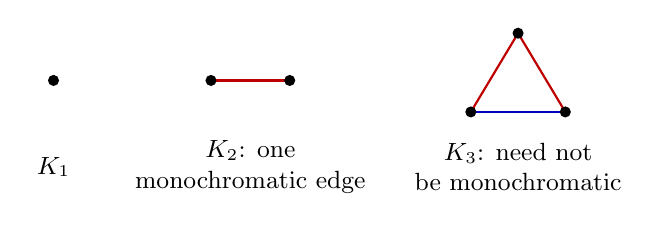
\begin{tikzpicture}[thick, every node/.style={font=\small}]
        \fill (0,0.4) circle (2pt);
        \node at (0,-0.7) {$K_1$};
        \draw[red!75!black] (2,0.4) -- (3,0.4);
        \fill (2,0.4) circle (2pt);
        \fill (3,0.4) circle (2pt);
        \node[align=center] at (2.5,-0.7) {$K_2$: one\\monochromatic edge};
        \draw[red!75!black] (5.3,0) -- (5.9,1) -- (6.5,0);
        \draw[blue!75!black] (5.3,0) -- (6.5,0);
        \foreach \point in {(5.3,0),(5.9,1),(6.5,0)} \fill \point circle (2pt);
        \node[align=center] at (5.9,-0.7) {$K_3$: need not\\be monochromatic};
    \end{tikzpicture}
\end{center}

We can first show \(R(3) > 5\) by giving an example: 
\begin{center}
    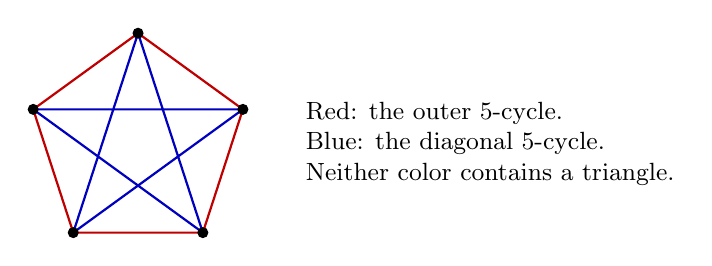
\begin{tikzpicture}[thick, every node/.style={font=\small}]
        \foreach \index in {1,...,5}
            \coordinate (pentagon-\index) at ({90-72*(\index-1)}:1.4);
        \draw[red!75!black] (pentagon-1) -- (pentagon-2) -- (pentagon-3)
            -- (pentagon-4) -- (pentagon-5) -- cycle;
        \draw[blue!75!black] (pentagon-1) -- (pentagon-3) -- (pentagon-5)
            -- (pentagon-2) -- (pentagon-4) -- cycle;
        \foreach \index in {1,...,5} \fill (pentagon-\index) circle (2pt);
        \node[align=left, anchor=west] at (2,0)
            {Red: the outer $5$-cycle.\\Blue: the diagonal $5$-cycle.\\Neither color contains a triangle.};
    \end{tikzpicture}
\end{center}

We can also show \(R(3) \le 6\) by pigeonhole principle: Consider \(K_6\) with vertices indexed by \(1, 2, 3, 4, 5, 6\), we know there exists 3 edges incident to vertex 1 are of same colors, WLOG, say vertices 2, 3, 4 are of red. Then we can show that no matter how we color \(\left\{ 2, 3 \right\}, \left\{ 3, 4 \right\}, \left\{ 2, 4 \right\}   \), there must be a monochromatic triangle.  

\begin{center}
    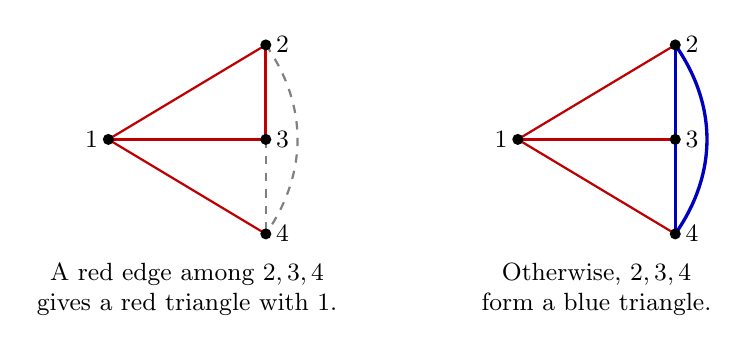
\begin{tikzpicture}[thick, every node/.style={font=\small}]
        \foreach \offset/\case in {0/1,5.2/2} {
            \begin{scope}[xshift=\offset cm]
                \coordinate (root) at (0,0);
                \foreach \index/\height in {2/1.2,3/0,4/-1.2} {
                    \coordinate (neighbor-\index) at (2,\height);
                    \draw[red!75!black] (root) -- (neighbor-\index);
                }
                \ifnum\case=1
                    \draw[red!75!black, very thick] (neighbor-2) -- (neighbor-3);
                    \draw[gray, dashed] (neighbor-3) -- (neighbor-4);
                    \draw[gray, dashed] (neighbor-2) to[bend left=35] (neighbor-4);
                    \node[align=center] at (1,-1.9) {A red edge among $2,3,4$\\gives a red triangle with $1$.};
                \else
                    \draw[blue!75!black, very thick] (neighbor-2) -- (neighbor-3) -- (neighbor-4);
                    \draw[blue!75!black, very thick] (neighbor-2) to[bend left=35] (neighbor-4);
                    \node[align=center] at (1,-1.9) {Otherwise, $2,3,4$\\form a blue triangle.};
                \fi
                \fill (root) circle (2pt) node[left] {$1$};
                \foreach \index in {2,3,4}
                    \fill (neighbor-\index) circle (2pt) node[right] {$\index$};
            \end{scope}
        }
    \end{tikzpicture}
\end{center}
Only the relevant edges are shown; vertices \(5,6\) and all other edges can be ignored. Hence every red-/blue-coloring of \(K_6\) has a monochromatic triangle, so \(R(3)=6\).

\begin{theorem}[Erdos-Szekeres, 1935]
    \[
        R(k) \le 4^k.
    \] 
\end{theorem}

\begin{proof}
    Let \(k\ge 2\), and consider any red-/blue-coloring of \(K_{2^{2k}}\). Set \(V_0=V(K_{2^{2k}})\). We successively choose vertices \(v_1,v_2,\ldots\), colors \(c_1,c_2,\ldots\), and nested sets \(V_0\supseteq V_1\supseteq V_2\supseteq\cdots\).

    At step \(i\), choose \(v_i\in V_{i-1}\). Among the edges from \(v_i\) to \(V_{i-1}\setminus\{v_i\}\), at least half have the same color, say \(c_i\). Let \(V_i\) be the set of endpoints of these edges. Then every edge from \(v_i\) to \(V_i\) has color \(c_i\), and
    \[
        |V_i|\ge \left\lceil\frac{|V_{i-1}|-1}{2}\right\rceil
        \ge 2^{2k-i}.
    \]
    The last inequality follows inductively from \(|V_0|=2^{2k}\); the ceiling accounts for removing \(v_i\) before keeping a color class.

    \begin{center}
        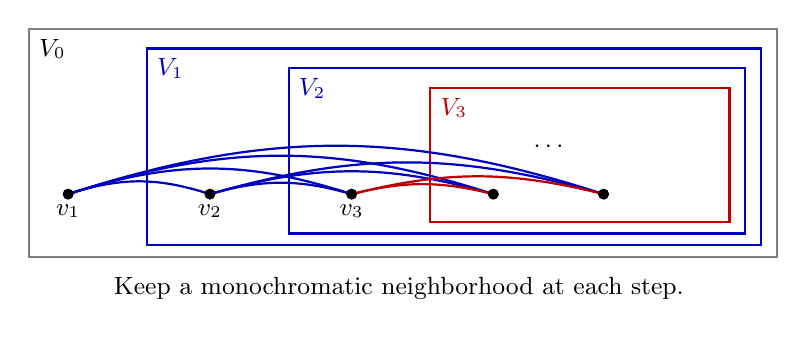
\begin{tikzpicture}[thick, every node/.style={font=\small}]
            \draw[gray] (-0.5,-0.8) rectangle (9,2.1);
            \draw[blue!75!black] (1,-0.65) rectangle (8.8,1.85);
            \draw[blue!75!black] (2.8,-0.5) rectangle (8.6,1.6);
            \draw[red!75!black] (4.6,-0.35) rectangle (8.4,1.35);
            \node[anchor=north west] at (-0.5,2.1) {$V_0$};
            \node[blue!75!black, anchor=north west] at (1,1.85) {$V_1$};
            \node[blue!75!black, anchor=north west] at (2.8,1.6) {$V_2$};
            \node[red!75!black, anchor=north west] at (4.6,1.35) {$V_3$};
            \coordinate (chosen-1) at (0,0);
            \coordinate (chosen-2) at (1.8,0);
            \coordinate (chosen-3) at (3.6,0);
            \foreach \target in {1.8,3.6,5.4,6.8}
                \draw[blue!75!black] (chosen-1) to[bend left=18] (\target,0);
            \foreach \target in {3.6,5.4,6.8}
                \draw[blue!75!black] (chosen-2) to[bend left=16] (\target,0);
            \foreach \target in {5.4,6.8}
                \draw[red!75!black] (chosen-3) to[bend left=14] (\target,0);
            \foreach \index in {1,2,3}
                \fill (chosen-\index) circle (2pt) node[below] {$v_\index$};
            \foreach \target in {5.4,6.8} \fill (\target,0) circle (2pt);
            \node at (6.1,0.6) {$\cdots$};
            \node at (4.2,-1.2) {Keep a monochromatic neighborhood at each step.};
        \end{tikzpicture}
    \end{center}

    In particular, for \(j<\ell\le i\), we have \(v_\ell\in V_j\), so the edge \(v_jv_\ell\) has color \(c_j\). Also, every edge from \(v_j\) to \(V_i\) has color \(c_j\).

    Repeat until \(i=2k\). This is possible since \(|V_{2k-1}|\ge 2\), and hence \(V_{2k}\) still contains at least one vertex. We obtain
    \[
        \begin{array}{c|cccccc}
            \text{vertex} & v_1 & v_2 & v_3 & \cdots & v_{2k-1} & v_{2k} \\
            \text{color} & c_1 & c_2 & c_3 & \cdots & c_{2k-1} & c_{2k}
        \end{array}
    \]
    By the pigeonhole principle, at least \(k\) of the colors \(c_1,\ldots,c_{2k}\) are equal. Choose indices \(i_1<\cdots<i_k\) with this common color. For any \(r<s\), the edge \(v_{i_r}v_{i_s}\) has color \(c_{i_r}\), so these \(k\) vertices form a monochromatic \(K_k\). Thus \(R(k)\le 2^{2k}=4^k\). The case \(k=1\) is immediate.
\end{proof}

\begin{remark}
    More careful counting gives \(R(k) \le \binom{2k - 2}{k - 1}\). 
\end{remark}

For the lower bound, we can use a smart construction to show \(R(k) > (k - 1)^2\):
For \(k\ge 2\), partition the vertices of \(K_{(k-1)^2}\) into \(k-1\) parts \(V_1,\ldots,V_{k-1}\), each of size \(k-1\). Color all edges inside a part blue and all edges between different parts red.
\begin{center}
    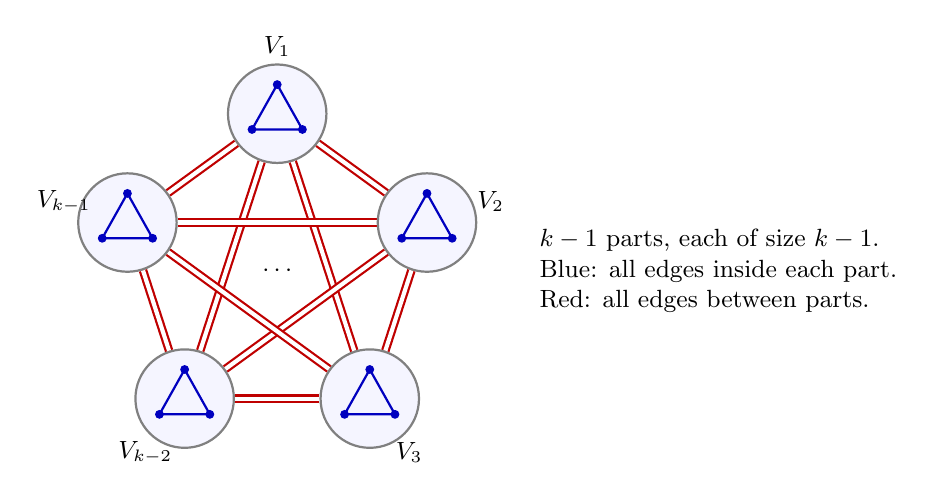
\begin{tikzpicture}[thick, every node/.style={font=\small}]
        \foreach \index in {1,...,5}
            \node[circle, minimum size=1.25cm, inner sep=0pt] (part-\index)
                at ({90-72*(\index-1)}:2) {};
        \foreach \first in {1,...,4} {
            \pgfmathtruncatemacro{\nextindex}{\first+1}
            \foreach \second in {\nextindex,...,5}
                \draw[red!75!black, double, double distance=1.5pt] (part-\first) -- (part-\second);
        }
        \foreach \index/\partlabel in {1/1,2/2,3/3,4/{k-2},5/{k-1}} {
            \begin{scope}[shift={(part-\index.center)}]
                \filldraw[fill=blue!4, draw=gray] (0,0) circle (0.625);
                \draw[blue!75!black] (0,0.37) -- (-0.32,-0.2) -- (0.32,-0.2) -- cycle;
                \foreach \point in {(0,0.37),(-0.32,-0.2),(0.32,-0.2)}
                    \fill[blue!75!black] \point circle (1.6pt);
            \end{scope}
            \node at ({90-72*(\index-1)}:2.85) {$V_{\partlabel}$};
        }
        \node[fill=white, inner sep=3pt] at (0,0) {$\cdots$};
        \node[align=left, anchor=west] at (3.2,0)
            {$k-1$ parts, each of size $k-1$.\\Blue: all edges inside each part.\\Red: all edges between parts.};
    \end{tikzpicture}
\end{center}
The diagram is schematic: each circle represents an entire blue \(K_{k-1}\), and each red connection represents all edges between two parts. A blue clique must lie in a single part, so it has at most \(k-1\) vertices. A red clique contains at most one vertex from each part, so it also has at most \(k-1\) vertices. Thus this coloring has no monochromatic \(K_k\), proving \(R(k)>(k-1)^2\).

\begin{theorem}[Erdos, 1947]
    \[
        R(k) > (\sqrt{2} - o(1))^k = 2^{\left( \frac{1}{2} - o(1) \right) k}.
    \] 
\end{theorem}

\begin{proof}
    Take the complete graph \(K_n\) on \(n\) vertices. Coloring each edge red or blue with probability \(\frac{1}{2}\), independently. 

    The bad events, say \(E_S\), is the event that set \(S\) of \(k\) vertices whose edges are all the same color. Then 
    \[
        \mathbb{P} (E_S) = 2 \cdot \left( \frac{1}{2} \right)^{\binom{k}{2}}.
    \]      

    Then 
    \begin{align*}
        \mathbb{P} \left( \text{coloring is bad}  \right) &= \mathbb{P} \left( \bigcup_{S \in \binom{V}{k}} E_S  \right) \le \sum_{S \in \binom{V}{k}} \mathbb{P} (E_S) = \binom{n}{k} 2 \left( \frac{1}{2} \right)^{\binom{k}{2}} < 2 n^k 2^{- \frac{k(k-1)}{2}} \\
        &= 2 \left( \frac{n}{2^{\frac{k-1}{2}}} \right)^k. 
    \end{align*}

    If \(n < (1 - c) 2^{\frac{k-1}{2}}\) for some constant \(c > 0\), then 
    \[
        \mathbb{P} \left( \text{bad coloring}  \right) \le 2(1 - c)^k \to 0,  
    \]  
    and thus 
    \[
        \mathbb{P} \left( \text{coloring has no monochromatic } K_k  \right) > 0, 
    \]
    i.e. \(\exists \) a coloring of \(K_n\) without monochromatic \(K_k\). Hence, we must have \(R(k) > n\).    
\end{proof}

\begin{theorem}
    \[
        2^{\frac{1}{2} k} \lesssim R(k) \le 2^{2k}.
    \]
\end{theorem}

\begin{definition}[Extremal problem]
    An \vocab{extremal problem} is a problem to find the size of  a largest structure with a desired property.
\end{definition}

To solve such problem, we should 
\begin{enumerate}[(1)]
    \item show a structure of large size with given property. (lower bound)
    \item prove that larger structures can't have property. (upper bound)
\end{enumerate}

\begin{definition}[Probabilistic method]
    To use \vocab{probabilistic method} to solve a problem, you should construct a probability space on the set of structures, then show that the desired property has positive parts, which shows the existence of a structure with such property.
\end{definition}